\let\lesson\undefined
\newcommand{\lesson}{\phantomlesson{Bài 22 + 23.}}
\setcounter{section}{2}
\section{Trắc nghiệm}
\ANSMCQ
{	\begin{center}
		\begin{tabular}{|m{2.8em}|m{2.8em}|m{2.8em}|m{2.8em}|m{2.8em}|m{2.8em}|m{2.8em}|m{2.8em}|m{2.8em}|m{2.8em}|}
			\hline
			1.B  & 2.D  & 3.C  & 4.D  & 5.C  & 6.A  &7.D   &8.D  &9.B & 10.A \\
			\hline
			
		\end{tabular}
	\end{center}
}
\begin{enumerate}[label=\bfseries Câu \arabic*:, leftmargin=1.5cm]
	\item\mkstar{1}\\
	{Hình bên mô tả đồ thị lực tác dụng - độ biến dạng của một vật rắn. Giới hạn đàn hồi của vật là điểm nào trên đồ thị?
	\begin{center}
		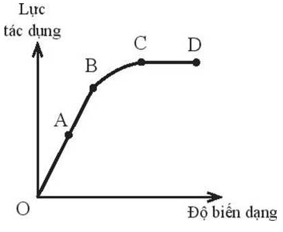
\includegraphics[width=0.3\linewidth]{../figs/VN10-2023-PH-TP033-2}
	\end{center}
\begin{mcq}(4)
	\item Điểm A.
	\item Điểm B.
	\item Điểm C.
	\item Điểm D.
\end{mcq}
}
\hideall{
\textbf{Đáp án B.}
}
	
	\item\mkstar{1}\\
	{Chọn phát biểu \textbf{sai} về lực đàn hồi của lò xo?
	\begin{mcq}
		\item Lực đàn hồi của lò xo có xu hướng chống lại nguyên nhân gây ra biến dạng.
		\item Lực đàn hồi của lò xo dài có phương là trục lò xo, chiều ngược với chiều biến dạng của lò xo.
		\item Lực đàn hồi của lò xo có độ lớn tuân theo định luật Hooke.
		\item Lực đàn hồi của lò xo chỉ xuất hiện ở đầu lò xo đặt ngoại lực gây biến dạng.
	\end{mcq}
}
\hideall{
\textbf{Đáp án D.}
}

\item \mkstar{2}\\
{Phải treo một vật có trọng lượng bằng bao nhiêu vào một lò xo có độ cứng $k =\SI{100}{\newton/\meter}$ để nó dãn ra được $\SI{10}{\centi\meter}$. Lấy $g =\SI{10}{\meter/\second^2}$.
\begin{mcq}(4)
	\item $\SI{1000}{\newton}$.
	\item $\SI{100}{\newton}$.
	\item $\SI{10}{\newton}$.
	\item $\SI{1}{\newton}$.
\end{mcq}
}
\hideall{
\textbf{Đáp án C.}\\
Trọng lượng vật cần treo:
$$P=F_\text{đh}=k\left|\Delta\ell\right|=\left(\SI{100}{\newton/\meter}\right)\cdot\left(\SI{0.1}{\meter}\right)=\SI{10}{\newton}.$$
}

	
	\item \mkstar{2}
	
	
	{
		Khi nói về lực đàn hồi của lò xo, phát biểu nào sau đây \textbf{sai?}
		\begin{mcq}
			\item Lực đàn hồi luôn có chiều ngược với chiều biến dạng của lò xo.
			\item Trong giới hạn đàn hồi, lực đàn hồi luôn tỉ lệ thuận với độ biến dạng.
			\item Khi lò xo bị dãn, lực đàn hồi có phương dọc theo trục lò xo.
			\item Lò xo luôn lấy lại được hình dạng ban đầu khi thôi tác dụng lực.
		\end{mcq}
	}
	
	\hideall
	{	
		\textbf{Đáp án: D.}
		
		Lò xo chỉ lấy lại được hình dạng ban đầu khi bị biến dạng trong giới hạn đàn hồi.
	}
	\item \mkstar{2}
	
	
	{
		Một vật có khối lượng $\SI{200}{g}$ được treo vào một lò xo thẳng đứng thì chiều dài của lò xo là $\SI{20}{cm}$. Biết khi chưa treo vật thì lò xo dài $\SI{18}{cm}$. Lấy $g=\SI{10}{m/s^2}$. Độ cứng của lò xo này là
		\begin{mcq}(4)
			\item $\SI{200}{N/m}$.
			\item $\SI{150}{N/m}$.
			\item $\SI{100}{N/m}$.
			\item $\SI{50}{N/m}$.
		\end{mcq}
	}
	
	\hideall
	{	
		\textbf{Đáp án: C.}
		
		Khi lò xo treo thẳng đứng thì
		$$k|\Delta l| = mg \Rightarrow k =\dfrac{mg}{\Delta l} = \SI{100}{N/m}$$
	}
	\item \mkstar{2}
	
	
	{
		Hai lò xo A và B có chiều dài tự nhiên bằng nhau. Độ cứng của lò xo A là $\SI{100}{N/m}$. Khi kéo hai lò xo với cùng lực $F$ thì lò xo A dãn $\SI{2}{cm}$, lò xo B dãn $\SI{1}{cm}$. Độ cứng của lò xo B là
		\begin{mcq}(4)
			\item $\SI{200}{N/m}$.
			\item $\SI{150}{N/m}$.
			\item $\SI{100}{N/m}$.
			\item $\SI{50}{N/m}$.
		\end{mcq}
	}
	
	\hideall
	{	
		\textbf{Đáp án: A.}
		
		Lập tỉ lệ:
		$$\dfrac{k_\text A}{k_\text B} = \dfrac{|\Delta \ell_\text B|}{|\Delta \ell_\text A|} \Rightarrow k_\text{B} = \SI{200}{N/m}$$
	}
	
	\item \mkstar{2}
	
	
	{
		Một lò xo nằm ngang có chiều dài tự nhiên là $\SI{40}{cm}$, khi bị nén lò xo dài $\SI{35}{cm}$ và lực đàn hồi khi đó bằng $\SI{2}{N}$. Khi lò xo bị nén với lực có độ lớn $\SI{5}{N}$ dọc theo trục lò xo thì lò xo có chiều dài
		\begin{mcq}(4)
			\item $\SI{35}{cm}$.
			\item $\SI{32.5}{cm}$.
			\item $\SI{25}{cm}$.
			\item $\SI{27.5}{cm}$.
		\end{mcq}
	}
	
	\hideall
	{	
		\textbf{Đáp án: D.}	
		
		Lập tỉ số:
		$$\dfrac{F_\text{đh 1}}{F_\text{đh 2}} = \dfrac{|\Delta \ell_1|}{|\Delta \ell_2|} \Rightarrow |\Delta \ell_2| = \SI{12.5}{cm}$$
		
		Vậy $\ell_2 =\ell_0-\left|\Delta\ell_2\right|= \SI{27.5}{cm}$.
	}
	\item \mkstar{3}
	
	
	{
		Một lò xo đầu trên gắn cố định. Nếu treo vật nặng khối lượng $\SI{600}{g}$ vào một đầu còn lại của lò xo thì lò xo có chiều dài $\SI{23}{cm}$. Nếu treo thêm vật nặng $\SI{800}{g}$ thì lò xo có chiều dài $\SI{24}{cm}$. Biết khi treo cả hai vật trên thì lò xo vẫn ở trong giới hạn đàn hồi. Lấy $g=\SI{10}{m/s^2}$. Độ cứng của lò xo là
		\begin{mcq}(4)
			\item $\SI{200}{N/m}$.
			\item $\SI{400}{N/m}$.
			\item $\SI{600}{N/m}$.
			\item $\SI{800}{N/m}$.
		\end{mcq}
	}
	
	\hideall
	{	
		\textbf{Đáp án: D.}
		
		Khi treo vật có $m_1=\SI{0.6}{kg}$ thì $\ell_1 = \ell_0 + \Delta \ell_1 = \SI{23}{cm}$. Suy ra:
		
		$$\ell_0 = \ell_1 - \dfrac{m_1 g}{k}$$
		
		Khi treo 2 vật có $m_1+m_2 = \SI{1.4}{kg}$ thì $\ell_2 = \ell_0 + \Delta \ell_2 = \SI{24}{cm}$. Suy ra:
		
		$$\ell_0 = \ell_2 - \dfrac{(m_1+m_2)g}{k}$$
		
		Vậy $$\ell_1 - \dfrac{m_1 g}{k} =\ell_2 - \dfrac{(m_1+m_2)g}{k} \Rightarrow k = \SI{800}{N/m} $$
	}
	
	
	\item\mkstar{3}\\
	{Một lò xo có độ cứng $\SI{80}{\newton/\meter}$ được treo thẳng đứng. Khi móc vào đầu tự do của nó một vật có khối lượng $\SI{400}{\gram}$ thì lò xo dài $\SI{18}{\centi\meter}$. Hỏi khi chưa móc vật thì lò xo dài bao nhiêu? Lấy $g =\SI{10}{\meter/\second^2}$.
	\begin{mcq}(4)
		\item $\SI{17.5}{\centi\meter}$.
		\item $\SI{13}{\centi\meter}$.
		\item $\SI{23}{\centi\meter}$.
		\item $\SI{18.5}{\centi\meter}$.
	\end{mcq}
}
\hideall{
\textbf{Đáp án B.}\\
Độ biến dạng của lò xo:
$$\left|\Delta\ell\right|=\dfrac{mg}{k}=\dfrac{\left(\SI{0.4}{\kilogram}\right)\cdot\left(\SI{10}{\meter/\second^2}\right)}{\SI{80}{\newton/\meter}}=\SI{0.05}{\meter}=\SI{5}{\centi\meter}$$
Khi chưa móc vật, chiều dài của lò xo:
$$\ell_0=\ell-\left|\Delta\ell\right|=\SI{13}{\centi\meter}.$$
}

\item \mkstar{3}\\
{Một lò xo có độ cứng $k$, có chiều dài tự nhiên $\ell_0$ một đầu giữ cố định ở A đầu kia gắn vào quả cầu khối lượng $m$ có thể trượt không ma sát trên thanh $\left(\Delta\right)$ nằm ngang. Thanh $\left(\Delta\right)$ quay đều với tốc độ góc $\omega$ quanh trục $\left(\Delta\right)$ thẳng đứng. Tính độ dãn của lò xo khi $\ell_0 =\SI{20}{\centi\meter}$, $\omega=\xsi{20\pi}{\radian/\second}$, $m =\SI{10}{\gram}$, $k =\SI{200}{\newton/\meter}$.
	\begin{center}
		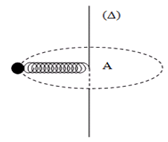
\includegraphics[width=0.3\linewidth]{../figs/VN10-2023-PH-TP033-3}
	\end{center}
\begin{mcq}(4)
	\item $\SI{5}{\centi\meter}$.
	\item $\SI{3.5}{\centi\meter}$.
	\item $\SI{6}{\centi\meter}$.
	\item $\SI{8}{\centi\meter}$.
\end{mcq}
}
\hideall{
\textbf{Đáp án A.}\\
Lực đàn hồi của lò xo đóng vai trò lực hướng tâm giữ cho vật chuyển động tròn đều:
$$F_\text{đh}=m\omega^2\left(\ell_0+\Delta\ell\right)$$
$$\Leftrightarrow k\cdot\Delta\ell=m\omega^2\left(\ell_0+\Delta\ell\right)$$
$$\Rightarrow \Delta\ell=\dfrac{\ell_0}{\dfrac{k}{m\omega^2}-1}\approx\SI{4.9}{\centi\meter}.$$
}
\end{enumerate}

\section{Tự luận}
\begin{enumerate}[label=\bfseries Câu \arabic*:]
	\item \mkstar{2}
	
	
	{
		Treo một vật có trọng lượng $\SI{2.0}{N}$ vào một cái lò xo, lò xo dãn ra $\SI{10}{mm}$. Treo một vật khác có trọng lượng chưa biết vào lò xo, nó dãn ra $\SI{80}{mm}$.
		\begin{enumerate}[label=\alph*)]
			\item Tính độ cứng của lò xo;
			\item Tính trọng lượng chưa biết.
		\end{enumerate}
	}
	
	\hideall
	{	
		\begin{enumerate}[label=\alph*)]
			\item Tính độ cứng của lò xo;
			
			Khi treo vật có trọng lượng $P_1=\SI{2.0}{N}$ thì $\Delta l_1 = \SI{10e-3}{m}$. Khi đó trọng lực và lưc đàn hồi cân bằng nên
			$$F_\text{đh 1} = P_1 = k |\Delta l_1| \Rightarrow k = \SI{200}{N/m}$$
			
			\item Tính trọng lượng chưa biết.
			
			$$P_2 = F_\text{đh 2} =k |\Delta l_2| = \SI{16}{N} $$
		\end{enumerate}
	}
	
	\item\mkstar{2}\\
	{Một học sinh thực hiện thí nghiệm đo độ cứng của một lò xo và thu được kết quả như hình. Độ cứng của lò xo này có giá trị bằng bao nhiêu?
		\begin{center}
			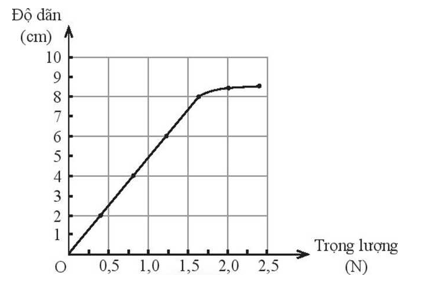
\includegraphics[width=0.4\linewidth]{../figs/VN10-2023-PH-TP033-4}
			\captionof{figure}{Kết quả thí nghiệm đo độ cứng lò xo.}
		\end{center}
	
}
\hideall{
Ta có:
$$F_\text{đh}=P$$
$$\Leftrightarrow k\Delta\ell=P$$
$$\Rightarrow k=\dfrac{P}{\Delta\ell}=\dfrac{\SI{1}{\newton}}{\SI{0.05}{\meter}}=\SI{20}{\newton/\meter}.$$
}
	
	\item \mkstar{3}
	
	
	{
		Một lò xo có độ cứng $\SI{100}{N/m}$ được treo thẳng đứng vào một điểm cố định, đầu dưới gắn với vật khối lượng $\SI{1}{kg}$. Vật được đặt trên giá đỡ D. Ban đầu giá đỡ D đứng yên và lò xo dãn $\SI{1}{cm}$. Cho D chuyển động nhanh dần đều hướng xuống với gia tốc $\SI{1}{m/s^2}$. Bỏ qua mọi ma sát và lực cản. Lấy $g=\SI{10}{m/s^2}$. Tính quãng đường mà giá đỡ đi được từ lúc bắt đầu chuyển động đến khi vật rời khỏi giá đỡ và tốc độ của vật khi đó.
	}
	
	\hideall
	{	
		Độ biến dạng của lò xo khi treo vật:
		$$\Delta \ell = \SI{10}{cm}$$
		Áp dụng định luật II Newton cho vật nặng trong quá trình lò xo dãn:
		$$\vec P+\vec N+\vec F_\text{đh}=m\vec a$$
		Chiếu phương trình định luật II Newton lên chiều trọng lực:
		$$P-N-F_\text{đh}=ma$$
		$$\Rightarrow N=P-F_\text{đh}-ma$$
		Khi vật nặng rời khỏi giá đỡ $N=0$:
		$$F_\text{đh}=m\left(g-a\right)\Rightarrow \Delta\ell=\dfrac{m\left(g-a\right)}{k}=\SI{0.09}{\meter}=\SI{9}{\centi\meter}$$
		Mà khi đặt trên D thì lò xo bị dãn $\SI{1}{cm}$, nên lò xo cần dãn thêm $\SI{8}{cm}$ nữa thì vật sẽ rời khỏi D.
		
		Vậy quãng đường mà D đi xuống thêm được là $s=\SI{8}{cm}$.
		
		Áp dụng công thức:
		$$v^2 -0 = 2aS \Rightarrow v = \SI{40}{cm/s}$$
	}

\item \mkstar{4}


{
	Một lò xo khối lượng không đáng kể, độ cứng $\SI{100}{N/m}$ và có chiều dài tự nhiên $\SI{40}{cm}$. Giữ đầu trên của lò xo cố định và buộc vào đầu dưới của lò xo một vật nặng khối lượng $\SI{500}{g}$, sau đó lại buộc thêm vào điểm chính giữa của lò xo đã bị dãn thêm một vật thứ hai khối lượng $\SI{500}{g}$. Lấy $g=\SI{10}{m/s^2}$. Tính chiều dài của lò xo khi đó.
}

\hideall
{	
	Chiều dài của lò xo khi treo vật thứ nhất:
	$$l_1 = l_0 + \Delta l_1 = l_0 + \dfrac{m_1g}{k} = \SI{45}{cm}$$
	
	Treo thêm vật thứ hai vào điểm chính giữa của lò xo đang dãn ($l_2 = \dfrac{l_1}{2} = \SI{22.5}{cm}$) thì tương ứng với cắt lò xo ra còn một nửa 
	$$k_1l_1= k_2 l_2 \Rightarrow k_2 = \dfrac{k_1l_1}{l_2} = \SI{200}{N/m}$$
	
	Độ biến dạng thêm của lò xo khi treo vật thứ hai:
	$$\Delta l_2 = \SI{2.5}{cm}$$
	
	Vậy với chiều dài khi theo vật thứ nhất là $\SI{45}{cm}$ mà còn biến dạng thêm một đoạn $\SI{2.5}{cm}$ thì chiều dài lò xo lúc này là $\SI{47.5}{cm}$
	
}
	
\end{enumerate}